\chapter{Outils de BruteForce}
\label{chap:BDD}

Après la phase de scan terminée, il sera sûrement nécessaire d'utiliser un outil de bruteforce afin de trouver un nouveau chemin d'attaque ou voir même d'obtenir un mot de passe permettant de terminer un CTF. Nous allons dans cette partie vous présenter dans un premier temps l'outil Dirb qui par son bruteforce permet de découvrir des répertoires ou des pages Web cachées. Puis, nous vous expliquerons le fonctionnement de John The Ripper qui permet de retrouver un hash.


\section{Dirbuster/Dirb}
\subsection{Définition}
Dirb est un scanneur de contenu web. Son but est de trouver l’existence d’objets web, qu’ils soient cachés ou non.
Son fonctionnement réside en la lancée d’une attaque par dictionnaire contre un serveur web et d’en analyser la réponse. \\
Cependant, il existe une différence entre attaque par dictionnaire et une attaque par bruteforce pure.\\
Une attaque par dictionnaire est une attaque que l’on utilise dans la cryptanalyse (technique de déduction d’un texte en clair par rapport à un texte chiffré sans la clé de chiffrement) pour justement trouver un mot de passe ou une clé de chiffrement. 
Son fonctionnement consiste à tester une liste donnée de mots de passe potentiels, un par un, en espérant que le mot de passe de chiffrement soit l’un deux. 
Cette technique ne marche donc pas systématiquement et il faut une énorme liste de mots de passe et du temps pour qu’elle soit efficace. L'intérêt d'installer des dictionnaires supplémentaires serait utile dans les cas de mots de passe très complexes.
C’est d’ailleurs à cause de ce genre d’attaque que l’on conseille de mettre des mots de passe compliqués, car ceux courants sont bien plus simples à trouver avec ce genre d’attaque. 
\subsection{Utilisation}
Pour le cas de Dirb, il est livré avec des dictionnaires de mots de passe pré-configurés, que l’on peut générer avec la commande : 
\begin{center}
    \textbf{html2dic}
\end{center}
En revanche, si l’on veut créer notre propre dictionnaire de mots, il faut utiliser la commande:
\begin{center}
    \textbf{gendict}
\end{center}
Cette commande crée une liste de mots incrémentaux qui vient d’un pattern que nous avons choisi, par exemple : 
\begin{center}
    \textbf{gendict -n Jean$_X$}
\end{center}
Ici, la valeur de X va changer en fonction du pattern que nous avons spécifié, soit -n, qui crée un pattern numérique, et donc notre liste de mots sera :
\begin{center}
    \textbf{Jean_1}\\
    \textbf{Jean_2}\\
    \textbf{Jean_3}\\
    \dots
\end{center}
On peut le faire aussi avec des lettres en mettant \textbf{-c}, des lettres en majuscule avec \textbf{-C}, ou encore de l'hexadécimal avec \textbf{-h}.
Quand la liste de mots est créée, elle est stockée ensuite dans
\textbf{/usr/share/wordlists/dirb/common.txt.}\\
\noindent Maintenant que la liste de mots est faite, il reste à trouver un site à attaquer, et quand cela est fait, il reste à faire la commande finale, qui va lancer l’attaque :\\
\begin{center}
\textbf{dirb https://www.nasa.gov/ /usr/share/wordlists/dirb/common.txt}
\end{center}
Dirb est surtout là pour faire des test de sécurité d’un site, de couvrir des trous non couverts par les scanneurs de vulnérabilités mais en aucun cas ne cherche des vulnérabilités.\\

\subsection{Comparaison entre Dirb et Dirbuster}
Pour ceux qui préfèrent les interfaces graphiques aux lignes de commandes, il existe l'équivalent de Dirb en GUI (Graphical User Interface), qui se nomme Dirbuster.\\

Ce dernier permet, lui aussi, d’attaquer un site par dictionnaire. Il suffit de rentrer l'adresse du site ainsi que le répertoire où est stocké la liste de mots de la manière suivante : 
\begin{figure}[htp!]
  \centering
  \setlength\figureheight{7cm}
  \setlength\figurewidth{9cm}
  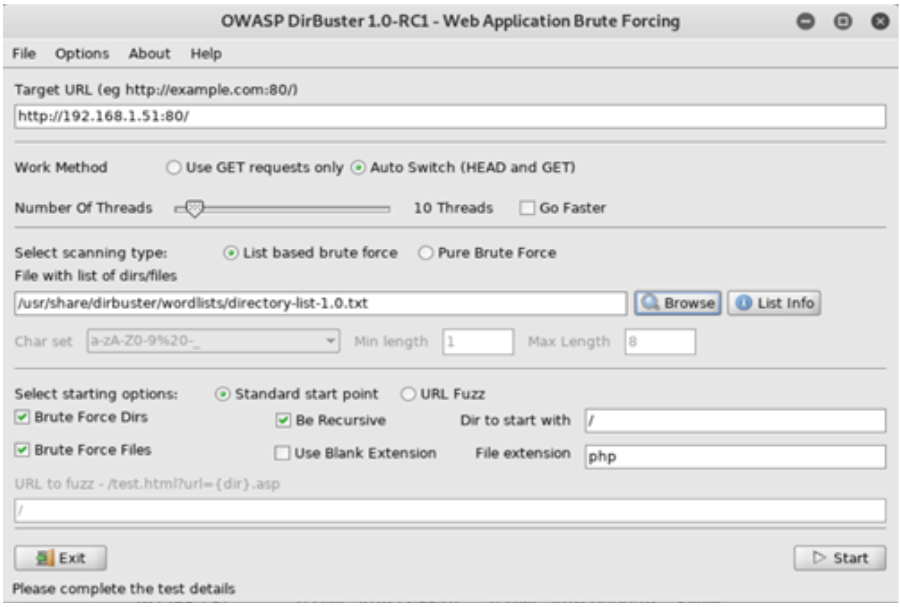
\includegraphics[width=0.8\textwidth]{oui/Screens/dirb1.PNG}
  \caption{Utilisation de dirbuster}
  \label{fig:courbe-tikz}
\end{figure}

\newpage
\noindent Ici, le site attaqué est \textbf{http://192.168.1.51} en utilisant la liste de mots située dans \textbf{/usr/share/dirbuster/wordlists/directory-list-1.0.txt}.\\ 
Dirbuster affiche ensuite les résultats de l’attaque : 
\begin{figure}[htp!]
  \centering
  \setlength\figureheight{7cm}
  \setlength\figurewidth{9cm}
  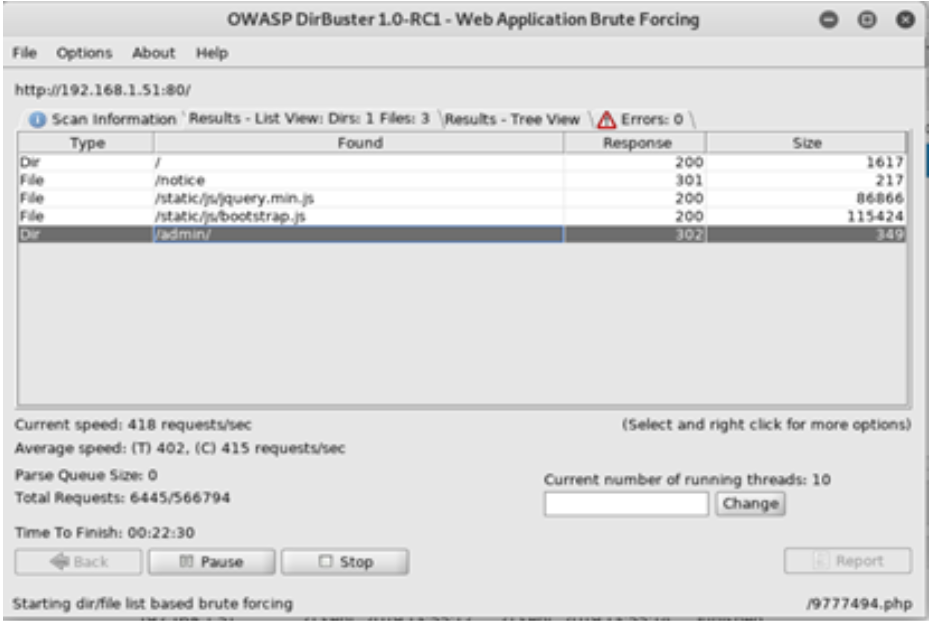
\includegraphics[width=0.8\textwidth]{oui/Screens/dirb2.PNG}
  \caption{Utilisation de dirbuster}
  \label{fig:courbe-tikz}
\end{figure}

L’utilisation de Dirb et Dirbuster est fondamentalement la même, mais ils ont chacun leurs avantages. 

Tout d’abord pour la question de rapidité, Dirb est en single-threading alors que Dirbuster est en multi-threading. 
La différence entre single et multi est qu’en single, on ne peut exécuter les tâches qu’une par une, de la manière suivante : 
\begin{center}
   \begin{figure}[htp!]
  \centering
  \setlength\figureheight{7cm}
  \setlength\figurewidth{9cm}
  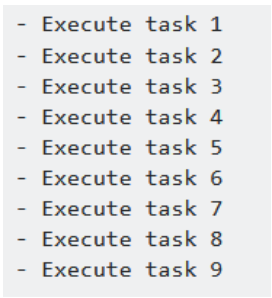
\includegraphics[width=0.3\textwidth]{oui/Screens/dirb3.PNG}
  \caption{Single-threading}
  \label{fig:courbe-tikz}
\end{figure} 
\end{center}

\newpage
Alors que le multi, lui, permet de faire plusieurs tâches en même temps en ordonnant les tâches en plusieurs threads, de la manière suivante : 
\begin{center}
    \textbf{Thread1}:\\
       \begin{figure}[htp!]
  \centering
  \setlength\figureheight{7cm}
  \setlength\figurewidth{9cm}
  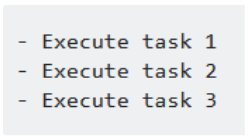
\includegraphics[width=0.3\textwidth]{oui/Screens/dirb4.PNG}
  \label{fig:courbe-tikz}
\end{figure}
\textbf{Thread2}:\\
       \begin{figure}[htp!]
  \centering
  \setlength\figureheight{7cm}
  \setlength\figurewidth{9cm}
  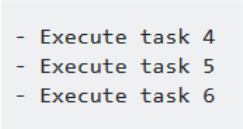
\includegraphics[width=0.3\textwidth]{oui/Screens/dirb5.PNG}
  \label{fig:courbe-tikz}
\end{figure}\\
\newpage
\textbf{Thread3}:\\
       \begin{figure}[htp!]
  \centering
  \setlength\figureheight{7cm}
  \setlength\figurewidth{9cm}
  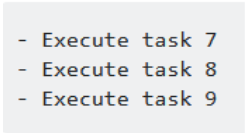
\includegraphics[width=0.3\textwidth]{oui/Screens/dirb6.PNG}
  \caption{Multi-threading}
  \label{fig:courbe-tikz}
\end{figure}
\end{center}
Il faut noter que la différence ne se voit qu’avec des processeurs multi-coeurs, qui peuvent faire plusieurs tâches à la fois. \\
Donc pour la rapidité d’exécution, si nous avons un bon processeur, Dirbuster surpasse totalement Dirb.\\
Seulement, Dirbuster demande toujours une interaction graphique, alors que Dirb, étant une CLI (Command Line Interface), permet l’automatisation, donc on perd certes du temps sur l’exécution des tâches mais on gagne du temps sur le reste.\\

\noindent \textbf{Conclusion}\\
En conclusion, Dirb et Dirbuster sont deux outils de scan très pratiques, notamment pour les CTFs car ils permettent de scanner les fichiers et dossiers du site ciblé. 

\section{John the Ripper}


\subsection{Définition}

John The Ripper ou plus communément, John, est un utilitaire multi-plates-formes ayant pour principal objectif de casser des mots de passe. John est certainement le programme le plus utilisé pour la sécurité de mot de passe.
John a plusieurs fonctionnalités. En effet, dans un premier temps, il est capable de reconnaître un hash donné. Cette fonctionnalité pourra nous être utile lors de CTF pour savoir comment recoder une information modifiée par exemple. Ensuite, en fonction du hash qu’il a reconnu et des options qu’on lui a associé, John est capable de trouver un mot de passe associé à un utilisateur.
Nous allons donc nous pencher sur son fonctionnement.

\subsection{Fonctionnement}

Comme nous l’avons vu dans la partie de Dirb, il existe une différence entre une attaque par dictionnaire et une attaque par bruteforce. Ici, John a la possibilité de faire 4 différents types d’attaques que nous allons détailler.

\subsubsection{Attaque via single mode}

Ce mode est le mode par défaut de cassage de mot de passe sur John. Cette attaque va tester tous les mots de passe basiques que nous avons l’habitude d’utiliser en fonction du nom d’utilisateur. Regardons un exemple très simple.
Nous allons hasher le mot de passe ‘ user1999 ‘ et ‘ salon ‘ pour les utilisateurs respectifs ‘ user1 ‘ et ‘ user2 ‘ via un site web.

Ensuite, nous allons enregistrer ceci dans un fichier texte sous ce format :

\begin{figure}[htp!]
  \centering
  \setlength\figureheight{7cm}
  \setlength\figurewidth{9cm}
  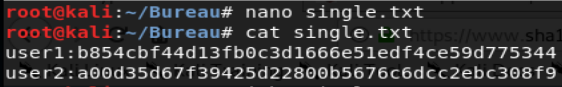
\includegraphics[width=1\textwidth]{oui/Screens/John/format_txt.PNG}
  \caption{Format d'utilisation pour John}
  \label{fig:courbe-tikz}
\end{figure}

Nous pouvons à présent lancer John sans option en lui précisant juste le fichier à attaquer puis observer le résultat de l’attaque :

\begin{figure}[htp!]
  \centering
  \setlength\figureheight{7cm}
  \setlength\figurewidth{9cm}
  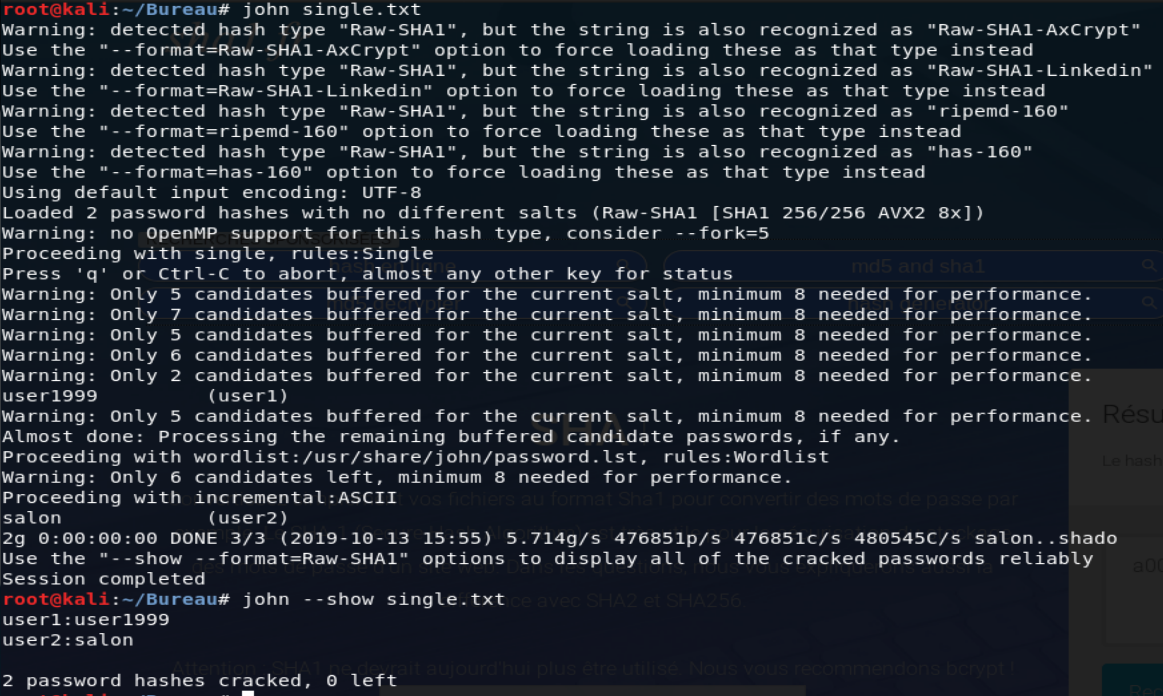
\includegraphics[width=1\textwidth]{oui/Screens/John/affichage_mdp_single.PNG}
  \caption{John par défaut}
  \label{fig:courbe-tikz}
\end{figure}

Dans un premier temps, on retrouve la première phase de John qui est l’analyse du hash. Il détecte dans notre cas que les mots de passe sont hashés en SHA1.
Il va alors essayer de reconnaître des mots de passe qu’il avait déjà trouvé à partir de cet hôte et des mots de passe ressemblants à l’utilisateur.
Puis dans une seconde partie, John n’a pas su trouver le mot de passe ‘salon’ associé à user2. Il a dû donc procéder à une attaque par mode incrémental. Pour éviter cela, on aurait pu forcer John à rester sur le single mode avec l'option ' --single '.


\subsubsection{Attaque par dictionnaire}

Comme nous l’avons vu avec l’outil Dirb, qui fait une attaque par dictionnaire, le principe sera ici le même. John va se baser sur un dictionnaire afin de trouver le mot de passe. En effet, le dictionnaire va être utilisé en fonction des règles que John aura reçues. Ainsi, si le mot de passe correspond aux règles combinées au dictionnaire, John pourra nous donner le mot de passe.
Nous allons essayer ce concept avec le dictionnaire ‘rockyou.txt’ fourni par Kali :

\begin{figure}[htp!]
  \centering
  \setlength\figureheight{7cm}
  \setlength\figurewidth{9cm}
  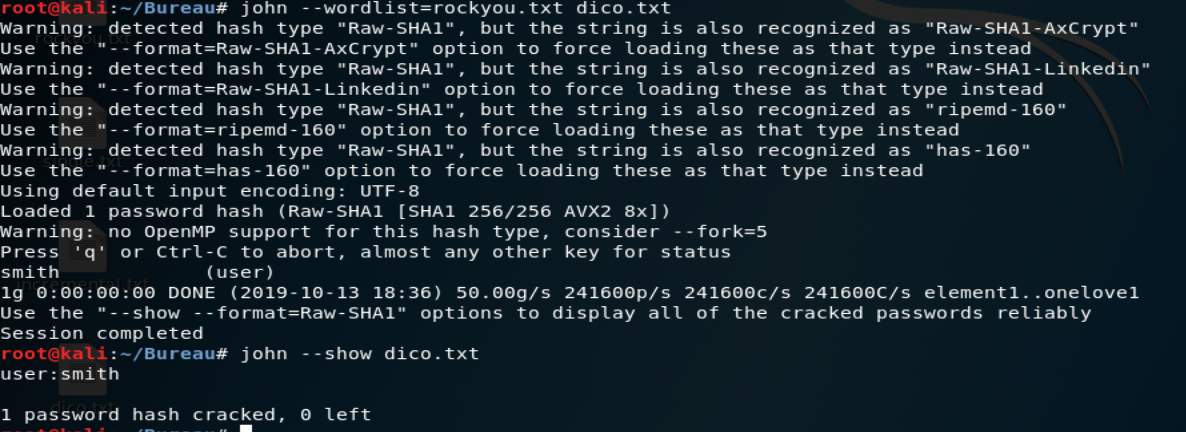
\includegraphics[width=1\textwidth]{oui/Screens/John/Dico.PNG}
  \caption{Attaque avec dictionnaire}
  \label{fig:courbe-tikz}
\end{figure}

L’attaque a été très rapide car le dictionnaire fourni par Kali est très complet.
    Nous pouvons maintenant voir l’attaque via le mode incrémental.

\subsubsection{Attaque via le mode incrémental}
Le mode incrémental est un mode permettant de tester toutes les combinaisons possibles afin d'arriver à nos fins. C’est le moyen ultime pour obtenir un mot de passe car il fonctionnera toujours. Mais il ne faudra pas être pressé car, plus le mot de passe sera long, plus ce mode prendra du temps.
Nous allons rajouter un ‘ user3 ‘ avec pour mot de passe ‘ velizy78 ’ pour que le mode simple soit incapable de le trouver. Nous allons juste indiquer à John d’utiliser directement le mode incrémental sans option.
Cependant, après plusieurs minutes, John n’avait pas trouvé et avait crashé.
Nous allons donc faciliter la recherche de John en lui annonçant que nous savons quels sont les types de caractères à rechercher. En effet, le mode incrémental a des options que nous allons observer.
L’option ‘ alpha ‘ va nous permettre de rechercher les mots de passe avec les lettres du clavier :

\begin{figure}[htp!]
  \centering
  \setlength\figureheight{7cm}
  \setlength\figurewidth{9cm}
  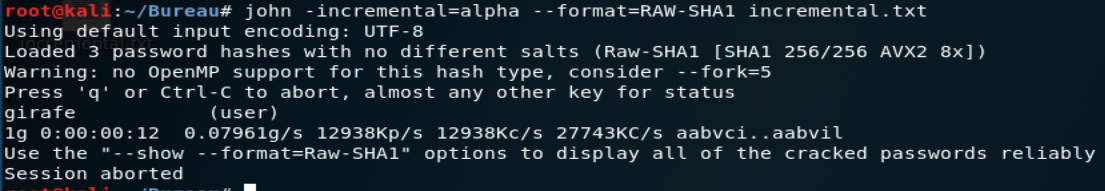
\includegraphics[width=1\textwidth]{oui/Screens/John/incremental_alpha.PNG}
  \caption{Attaque en mode incrémental alphabet}
  \label{fig:courbe-tikz}
\end{figure}

L’option "digit" va nous permettre de rechercher les mots de passe avec les chiffres du clavier :

\begin{figure}[htp!]
  \centering
  \setlength\figureheight{7cm}
  \setlength\figurewidth{9cm}
  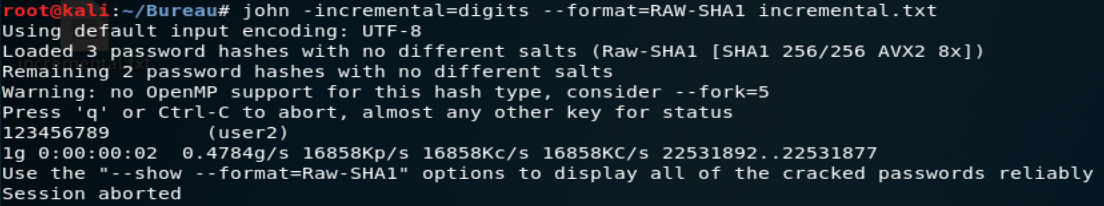
\includegraphics[width=1\textwidth]{oui/Screens/John/incremental_digits.PNG}
  \caption{Attaque en mode incrémental chiffre}
  \label{fig:courbe-tikz}
\end{figure}

L’option ‘ ASCII ‘ va nous permettre d’utiliser l'alphabet ASCII qui regroupe presque la totalité du clavier :

\begin{figure}[htp!]
  \centering
  \setlength\figureheight{7cm}
  \setlength\figurewidth{9cm}
  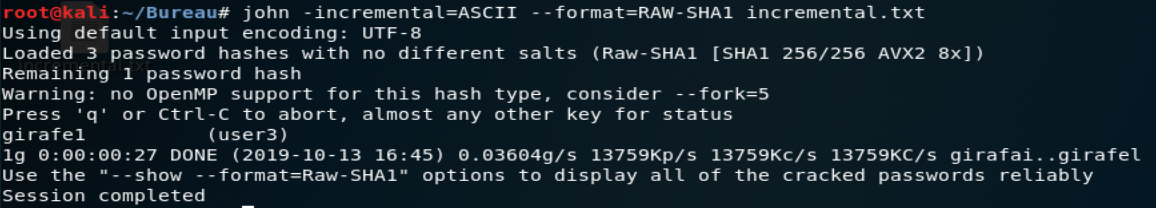
\includegraphics[width=1\textwidth]{oui/Screens/John/incremental_ASCII.PNG}
  \caption{Attaque en mode incrémental ASCII}
  \label{fig:courbe-tikz}
\end{figure}

Comme on peut le voir, plus le champ de recherche est important, plus le mot de passe prend du temps à être trouvé.